\section{Methods}
\label{sec:methods}

Before diving into the complex implementations and algorithms, it is essential we visualize the core concepts mentioned in the previous section.

\begin{Note} 
    All of these visualizations are created using my own TypeScript implementation of a simple graphics library built on top of the HTML5 Canvas API. The code for this library is available in the repository of this thesis, and the visualizations can be viewed in the browser here: \url{https://kisskonraduni.github.io/emergent-animations/examples}.
\end{Note}

\vspace{1cm}

\subsection{Visualizing Coordinate Systems and Transformations}
\label{sec:visualizing-coordinate-systems}

Understanding how objects are positioned and transformed requires a clear grasp of the different coordinate spaces used in graphics programming.

From here on, I recommend opening the interactive examples on a nearby device, as the visualizations will be referenced throughout the thesis. While still images are provided for most examples, seeing them in motion is ideal. Let's begin by examining the main coordinate spaces used in graphics programming.

\subsubsection{World Space}
\label{sec:world-space}

\begin{figure}[h]
    \centering
    \begin{minipage}[b]{0.4\textwidth}
        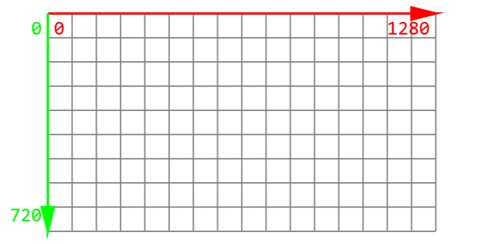
\includegraphics[width=\linewidth]{img/world-space.jpg}
        \caption{World Space Coordinate System \textbf{in my Graphics Library}}
    \end{minipage}\hfill
    \begin{minipage}[b]{0.55\textwidth}
        \setlength{\parskip}{1em}
        \setlength{\parindent}{0pt}
        World Space is the base coordinate system in a graphics library or game engine. The origin is at the top-left corner \textit{in my library}, with the x-axis pointing right and the y-axis pointing down. Almost all objects are positioned in this space, and transformations are applied relative to the origin.

        In this graphics library I have defined a \(\vec{\text{resolution}}=[1280, 720]\) vector, which is the area we see. 
    \end{minipage}
\end{figure}

\begin{Note}
    Technically speaking the \(\vec{\text{resolution}}\) vector is the bounds of an imaginary camera spanning from \([0, 0]\) to \([1280, 720]\). This variable is often used to define positions in the examples, as it makes our calculations easy to follow. The library always makes sure that with every resolution and aspect ratio this view is always centered and visible on the screen.
\end{Note}

\pagebreak

\subsubsection{Object Space}
\label{sec:object-space}

\begin{figure}[h]
    \centering
    \begin{minipage}[t]{0.35\textwidth}
        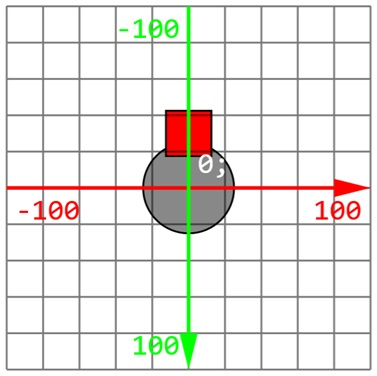
\includegraphics[width=\linewidth]{img/object-space.jpg}
        \caption{An example object with its Coordinate System visualized}
    \end{minipage}\hfill
    \begin{minipage}[b]{0.6\textwidth}
        \setlength{\parskip}{1em}
        \setlength{\parindent}{0pt}
        Object Space is the local coordinate system of an object, with the origin typically at the center. This space is used when defining the object's geometry and rendering. Transformations in Object Space are applied relative to the object's pivot point.

        This object has a tiny hat as a child element to visualize the local coordinate system of the object. The hat's position is set relative to the circle's pivot point, and moves with it. If we want the hat's position in World Space, we need to apply the object's transformations to the vector representing the hat's position.
    \end{minipage}
\end{figure}

\begin{Note}
    The pivot point is the reference for rotation and positioning within World Space. Correctly setting the pivot point is crucial: for UI elements, it allows easy anchoring; for game objects, such as a player character, the pivot is often set to the feet to ensure rotation occurs around the correct point.
\end{Note}

\vspace{1cm}

\subsubsection{Screen Space}
\label{sec:screen-space}

In this graphics library, Screen Space typically matches World Space, with the origin at the top-left corner. In 3D applications, an additional Camera Space is introduced: World Space $\rightarrow$ Camera Space $\rightarrow$ Screen Space. Camera Space represents the camera's position and orientation, while Screen Space is where the camera's view is projected, either at the top-left or center of the screen. This separation is important, as game objects and UI elements often exist in different spaces or layers.

\begin{Note}
    Using these transformations, we can create interactions between different spaces. For example, dragging an object in Screen Space can be transformed into World Space to update its position. Most 3D editors use a similar approach. This is possible thanks to the fact that the transformations can be done in reverse order, meaning we can transform a point from Screen Space to World Space, or from Object Space to World Space.
\end{Note}

\pagebreak
